\chapter{Was ist Hypertext?}
\label{ch:Was ist Hypertext?}

\begin{section}{Was ist überhaupt Hypertext?}
\label{sec:big_brother}

Was ist überhaupt Hypertext? Nach Jakob Nielsen in dem Buch Multimedia and Hpertext: The Internet and Beyond aus dem Jahr 1995, ist \glqq the simplest way to define hypertext is to contrast it with traditional text like a book. All traditional text, whether in printed form or in computer files, is sequential, meaning that there is a single linear sequence defining the order in which the text is to be read. [...] Hypertext is nonsequential; there is no single order that determines the sequence in which the text is to be read. [...]\grqq{ }\cite[S.1]{Nielsen1995}. Jakob Nielsen beschreibt, genau wie Jeff Conklin in seinem Artikel Hypertext: An Introduction and Survey, Hypertext als Informationsquelle die dem Leser die Freiheit gibt die Informationen in beliebiger Reihenfolge abzurufen. Der Leser dürfe entscheiden, welche Links er nutze und in welcher Reihenfolge \cite[S.33]{Conklin1987} \cite[S.1]{Nielsen1995}.

\begin{quote}
\glqq Hypertext allows and even encourages the writer to make such references, and allows the readers to make their own decisions about which links to follow and in what order. In this sense, hypertext eases the restrictions on the thinker and writer. It does not force a strict decision about whether any given idea is either within the flow of a paper's stream of thought or outside of it.\grqq{ }\cite[S.33]{Conklin1987}
\end{quote}

Also könnte ein Hypertext wie auf Abbildung \ref{fig:nielsenLink} zusehen, aus vielen einzelnen Informationen bestehen, zwischen denen eine Verlinkung existiert. Durch diese Links kann der Leser entscheiden an welcher Stelle er weiter lesen möchte. Anstatt eine den Text in der festen Reihenfolge $A$, $B$, $C$, $...$ und dann $G$ zu lesen, gibt es für den Leser mehrere Möglichkeiten die Texte aufzurufen. Nach Text $A$ könne zum Beispiel sofort Text $D$ folgen und so weiter\cite[S.1]{Nielsen1995}.

\begin{figure}[H]
	\centering
	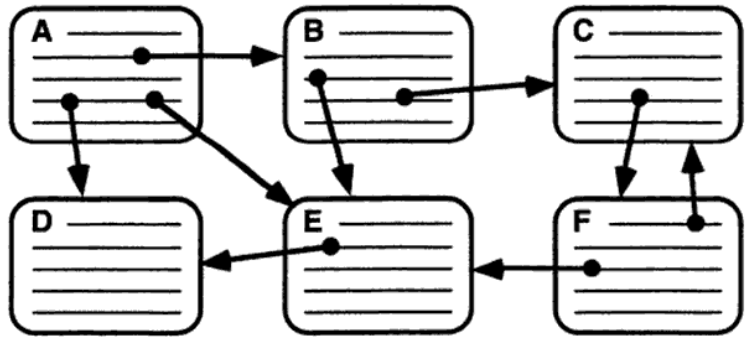
\includegraphics[width=0.8\textwidth]{image/nielsenLink}
	\caption{Vereinfachte Ansicht eines Hypertextes \cite[S.1]{Nielsen1995}}
	\label{fig:nielsenLink}
\end{figure}

Einen Hypertext kann oftmals als Graphen aus Knoten und Kanten dargestellt werden. Diese Darstellungsform kann vor dem Leser verborgen sein, muss es aber nicht \cite{Conklin1987}. Eine Information, ein Absatz, ein Text oder ein Dokument ist ein Knoten, die Größe spielt hierbei keine Rolle. Ein Knoten kann nun Links auf andere Knoten haben und diese sind dann die Kanten in dem Graphen \cite[S.19]{Conklin1987} \cite[S.2]{Nielsen1995}. Auch John B. Smith und Stephen F. Weiss schreiben in dem Artikel Hypertext vergleichbar über Hypertext als Netzwerk aus Informationen mit Links \cite{Smith1988}. Diese bezeichnen unteranderem auch Verlinkungen zwischen Medien wie Audio-, Grafik- oder Videodateien als Hypertext. In diesem Zusammenhang verwendet Ted Nelson auch den Begriff \glqq Hypermedia\grqq{ }\cite{Nelson1965}. 

\begin{quote}
    \glqq [...] Hypertext is an approach to information management in which data is stored in a network of nodes connected by links. Nodes can contain text, graphics, audio, video, as well as source code or other forms of data.\grqq{ }\cite{Smith1988}
\end{quote}

Wie auf Abbildung \ref{fig:imText} zu sehen, müsse eine Link also nicht unbedingt von Wort zu Wort führen, sondern sondern könne auch den Token $xxxx$ im Dokument $A$ mit dem ganze Dokument $B$ verbinden \cite{Conklin1987}. 

\begin{figure}[H]
	\centering
	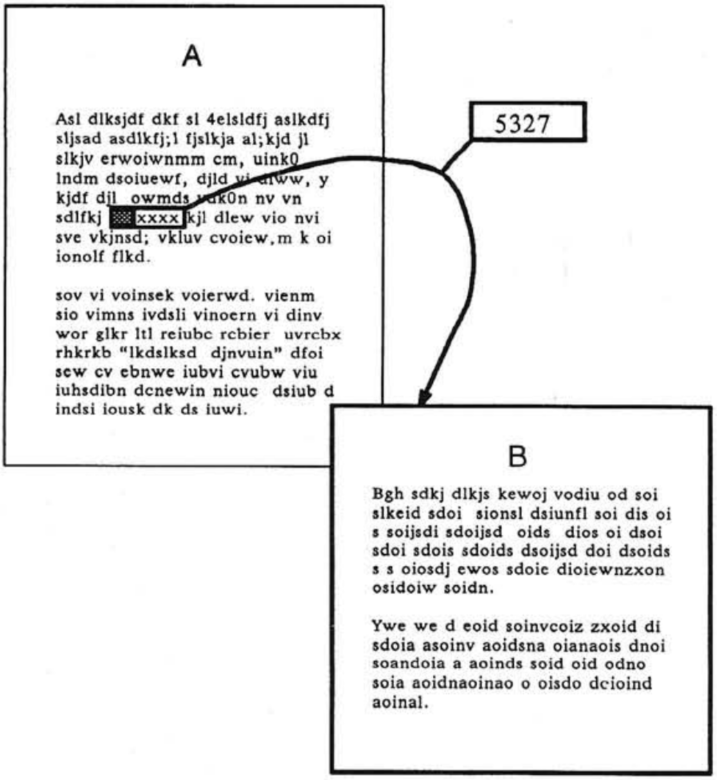
\includegraphics[width=0.8\textwidth]{image/imText}
	\caption{Ein Beispiel eines Links von in einem Text zu einem anderen Text \cite[S.34]{Conklin1987}}
	\label{fig:imText}
\end{figure}

\begin{quote}
    \glqq The same is true of footnotes in traditional printed texts, since readers have to determine upon reaching the footnote marker whether to continue reading the primary stream of text or to branch off to pursue the footnote. \grqq{ }\cite{Nielsen1995}
\end{quote}

Das gleiche könne auch auf einen traditionellen Text auf Papier zutreffen, Fußnoten referenzieren auf andere Texte und geben dem Leser die Möglichkeit an anderer Stelle weiterzulesen \cite{Nielsen1995}.

\end{section}

\begin{section}{Abgrenzung}
\label{sec:abgrenzung}

Doch für eine Antwort auf die Frage was ein Hypertext ist, gibt es sicherlich noch viele andere Antworten und Definitionen. Im Jahr 1945 wurde \glqq As we may think\grqq{ }von Vannevar Bush veröffentlicht. Dieses Konzept hierbei als Grundidee für Hypertext genutzt werden. Ich beschränke mich in dieser Arbeit auf lokale Hypertext-Systeme insbesondere der achtziger Jahre. Ich nehme in dieser Arbeit Bezug auf ausgewählte Hypertext-Systeme, deren Benutzung, Funktionen und technische Umsetzung. Ein besonderes Augenmerk legt diese Arbeit hierbei auf die Umsetzung der Links. Vernetzte und verteilte Hypertext-Systeme klammere ich in dieser Arbeit explizit aus.

\end{section}